\documentclass[twoside]{book}

% Packages required by doxygen
\usepackage{fixltx2e}
\usepackage{calc}
\usepackage{doxygen}
\usepackage[export]{adjustbox} % also loads graphicx
\usepackage{graphicx}
\usepackage[utf8]{inputenc}
\usepackage{makeidx}
\usepackage{multicol}
\usepackage{multirow}
\PassOptionsToPackage{warn}{textcomp}
\usepackage{textcomp}
\usepackage[nointegrals]{wasysym}
\usepackage[table]{xcolor}

% Font selection
\usepackage[T1]{fontenc}
\usepackage[scaled=.90]{helvet}
\usepackage{courier}
\usepackage{amssymb}
\usepackage{sectsty}
\renewcommand{\familydefault}{\sfdefault}
\allsectionsfont{%
  \fontseries{bc}\selectfont%
  \color{darkgray}%
}
\renewcommand{\DoxyLabelFont}{%
  \fontseries{bc}\selectfont%
  \color{darkgray}%
}
\newcommand{\+}{\discretionary{\mbox{\scriptsize$\hookleftarrow$}}{}{}}

% Page & text layout
\usepackage{geometry}
\geometry{%
  a4paper,%
  top=2.5cm,%
  bottom=2.5cm,%
  left=2.5cm,%
  right=2.5cm%
}
\tolerance=750
\hfuzz=15pt
\hbadness=750
\setlength{\emergencystretch}{15pt}
\setlength{\parindent}{0cm}
\setlength{\parskip}{3ex plus 2ex minus 2ex}
\makeatletter
\renewcommand{\paragraph}{%
  \@startsection{paragraph}{4}{0ex}{-1.0ex}{1.0ex}{%
    \normalfont\normalsize\bfseries\SS@parafont%
  }%
}
\renewcommand{\subparagraph}{%
  \@startsection{subparagraph}{5}{0ex}{-1.0ex}{1.0ex}{%
    \normalfont\normalsize\bfseries\SS@subparafont%
  }%
}
\makeatother

% Headers & footers
\usepackage{fancyhdr}
\pagestyle{fancyplain}
\fancyhead[LE]{\fancyplain{}{\bfseries\thepage}}
\fancyhead[CE]{\fancyplain{}{}}
\fancyhead[RE]{\fancyplain{}{\bfseries\leftmark}}
\fancyhead[LO]{\fancyplain{}{\bfseries\rightmark}}
\fancyhead[CO]{\fancyplain{}{}}
\fancyhead[RO]{\fancyplain{}{\bfseries\thepage}}
\fancyfoot[LE]{\fancyplain{}{}}
\fancyfoot[CE]{\fancyplain{}{}}
\fancyfoot[RE]{\fancyplain{}{\bfseries\scriptsize Generated by Doxygen }}
\fancyfoot[LO]{\fancyplain{}{\bfseries\scriptsize Generated by Doxygen }}
\fancyfoot[CO]{\fancyplain{}{}}
\fancyfoot[RO]{\fancyplain{}{}}
\renewcommand{\footrulewidth}{0.4pt}
\renewcommand{\chaptermark}[1]{%
  \markboth{#1}{}%
}
\renewcommand{\sectionmark}[1]{%
  \markright{\thesection\ #1}%
}

% Indices & bibliography
\usepackage{natbib}
\usepackage[titles]{tocloft}
\setcounter{tocdepth}{3}
\setcounter{secnumdepth}{5}
\makeindex

% Hyperlinks (required, but should be loaded last)
\usepackage{ifpdf}
\ifpdf
  \usepackage[pdftex,pagebackref=true]{hyperref}
\else
  \usepackage[ps2pdf,pagebackref=true]{hyperref}
\fi
\hypersetup{%
  colorlinks=true,%
  linkcolor=blue,%
  citecolor=blue,%
  unicode%
}

% Custom commands
\newcommand{\clearemptydoublepage}{%
  \newpage{\pagestyle{empty}\cleardoublepage}%
}

\usepackage{caption}
\captionsetup{labelsep=space,justification=centering,font={bf},singlelinecheck=off,skip=4pt,position=top}

%===== C O N T E N T S =====

\begin{document}

% Titlepage & ToC
\hypersetup{pageanchor=false,
             bookmarksnumbered=true,
             pdfencoding=unicode
            }
\pagenumbering{alph}
\begin{titlepage}
\vspace*{7cm}
\begin{center}%
{\Large R\+E\+MC\+: Replica exchange Monte Carlo }\\
\vspace*{1cm}
{\large Generated by Doxygen 1.8.13}\\
\end{center}
\end{titlepage}
\clearemptydoublepage
\pagenumbering{roman}
\tableofcontents
\clearemptydoublepage
\pagenumbering{arabic}
\hypersetup{pageanchor=true}

%--- Begin generated contents ---
\chapter{Namespace Index}
\section{Namespace List}
Here is a list of all documented namespaces with brief descriptions\+:\begin{DoxyCompactList}
\item\contentsline{section}{\hyperlink{namespacechecking__argument}{checking\+\_\+argument} }{\pageref{namespacechecking__argument}}{}
\item\contentsline{section}{\hyperlink{namespaceconformation}{conformation} }{\pageref{namespaceconformation}}{}
\item\contentsline{section}{\hyperlink{namespacemain}{main} }{\pageref{namespacemain}}{}
\item\contentsline{section}{\hyperlink{namespacemonte__carlo}{monte\+\_\+carlo} }{\pageref{namespacemonte__carlo}}{}
\end{DoxyCompactList}

\chapter{Hierarchical Index}
\section{Class Hierarchy}
This inheritance list is sorted roughly, but not completely, alphabetically\+:\begin{DoxyCompactList}
\item \contentsline{section}{Movement.\+Movement}{\pageref{classMovement_1_1Movement}}{}
\begin{DoxyCompactList}
\item \contentsline{section}{Corner\+\_\+moves.\+Corner\+\_\+moves}{\pageref{classCorner__moves_1_1Corner__moves}}{}
\item \contentsline{section}{Crankshaft\+\_\+moves.\+Crankshaft\+\_\+moves}{\pageref{classCrankshaft__moves_1_1Crankshaft__moves}}{}
\item \contentsline{section}{End\+\_\+moves.\+End\+\_\+moves}{\pageref{classEnd__moves_1_1End__moves}}{}
\item \contentsline{section}{Pull\+\_\+moves.\+Pull\+\_\+moves}{\pageref{classPull__moves_1_1Pull__moves}}{}
\end{DoxyCompactList}
\item \contentsline{section}{Residu.\+Residu}{\pageref{classResidu_1_1Residu}}{}
\end{DoxyCompactList}

\chapter{Class Index}
\section{Class List}
Here are the classes, structs, unions and interfaces with brief descriptions\+:\begin{DoxyCompactList}
\item\contentsline{section}{\hyperlink{classCorner__moves_1_1Corner__moves}{Corner\+\_\+moves.\+Corner\+\_\+moves} }{\pageref{classCorner__moves_1_1Corner__moves}}{}
\item\contentsline{section}{\hyperlink{classCrankshaft__moves_1_1Crankshaft__moves}{Crankshaft\+\_\+moves.\+Crankshaft\+\_\+moves} }{\pageref{classCrankshaft__moves_1_1Crankshaft__moves}}{}
\item\contentsline{section}{\hyperlink{classEnd__moves_1_1End__moves}{End\+\_\+moves.\+End\+\_\+moves} }{\pageref{classEnd__moves_1_1End__moves}}{}
\item\contentsline{section}{\hyperlink{classMovement_1_1Movement}{Movement.\+Movement} }{\pageref{classMovement_1_1Movement}}{}
\item\contentsline{section}{\hyperlink{classPull__moves_1_1Pull__moves}{Pull\+\_\+moves.\+Pull\+\_\+moves} }{\pageref{classPull__moves_1_1Pull__moves}}{}
\item\contentsline{section}{\hyperlink{classResidu_1_1Residu}{Residu.\+Residu} }{\pageref{classResidu_1_1Residu}}{}
\end{DoxyCompactList}

\chapter{Namespace Documentation}
\hypertarget{namespacechecking__argument}{}\section{checking\+\_\+argument Namespace Reference}
\label{namespacechecking__argument}\index{checking\+\_\+argument@{checking\+\_\+argument}}
\subsection*{Functions}
\begin{DoxyCompactItemize}
\item 
def \hyperlink{namespacechecking__argument_a3136d3e342a81821375edc2f731ce5f4}{check\+\_\+int\+\_\+type} (rep)
\item 
def \hyperlink{namespacechecking__argument_afe3bde94844d26f66c9a46cf08c4f1b3}{check\+\_\+arguments} (argv)
\end{DoxyCompactItemize}


\subsection{Detailed Description}
\begin{DoxyVerb}    Check if user enter all necessary arguments correctly.
    Otherwise, a message is sent to the user.
\end{DoxyVerb}
 

\subsection{Function Documentation}
\mbox{\Hypertarget{namespacechecking__argument_afe3bde94844d26f66c9a46cf08c4f1b3}\label{namespacechecking__argument_afe3bde94844d26f66c9a46cf08c4f1b3}} 
\index{checking\+\_\+argument@{checking\+\_\+argument}!check\+\_\+arguments@{check\+\_\+arguments}}
\index{check\+\_\+arguments@{check\+\_\+arguments}!checking\+\_\+argument@{checking\+\_\+argument}}
\subsubsection{\texorpdfstring{check\+\_\+arguments()}{check\_arguments()}}
{\footnotesize\ttfamily def checking\+\_\+argument.\+check\+\_\+arguments (\begin{DoxyParamCaption}\item[{}]{argv }\end{DoxyParamCaption})}

\begin{DoxyVerb}Assign options into variable and check if
option are correct.
    @param argv: Arguments given by the user
\end{DoxyVerb}
 \mbox{\Hypertarget{namespacechecking__argument_a3136d3e342a81821375edc2f731ce5f4}\label{namespacechecking__argument_a3136d3e342a81821375edc2f731ce5f4}} 
\index{checking\+\_\+argument@{checking\+\_\+argument}!check\+\_\+int\+\_\+type@{check\+\_\+int\+\_\+type}}
\index{check\+\_\+int\+\_\+type@{check\+\_\+int\+\_\+type}!checking\+\_\+argument@{checking\+\_\+argument}}
\subsubsection{\texorpdfstring{check\+\_\+int\+\_\+type()}{check\_int\_type()}}
{\footnotesize\ttfamily def checking\+\_\+argument.\+check\+\_\+int\+\_\+type (\begin{DoxyParamCaption}\item[{}]{rep }\end{DoxyParamCaption})}

\begin{DoxyVerb}Check if the answer can be cast into int
and return it
    @param rep: The answer given by the user in str
    Return the answer casted in int
\end{DoxyVerb}
 
\hypertarget{namespaceconformation}{}\section{conformation Namespace Reference}
\label{namespaceconformation}\index{conformation@{conformation}}
\subsection*{Functions}
\begin{DoxyCompactItemize}
\item 
def \hyperlink{namespaceconformation_a68e0c087ab604cbc37a7fe9a27622d8c}{vshd\+\_\+move} (index, structure\+\_\+grid, residues)
\item 
\mbox{\Hypertarget{namespaceconformation_aff463b8b684c4af25a3016b5e9bde9a7}\label{namespaceconformation_aff463b8b684c4af25a3016b5e9bde9a7}} 
def {\bfseries pullmoves\+\_\+move} (residu, structure\+\_\+grid)
\item 
\mbox{\Hypertarget{namespaceconformation_aff776064950617ef8272323343ef9a95}\label{namespaceconformation_aff776064950617ef8272323343ef9a95}} 
def {\bfseries mixe\+\_\+move} (residu, structure\+\_\+grid)
\end{DoxyCompactItemize}


\subsection{Detailed Description}
\begin{DoxyVerb}    Define different movement possible according to user's choice.
    Then, launch the most appropriate movement.
\end{DoxyVerb}
 

\subsection{Function Documentation}
\mbox{\Hypertarget{namespaceconformation_a68e0c087ab604cbc37a7fe9a27622d8c}\label{namespaceconformation_a68e0c087ab604cbc37a7fe9a27622d8c}} 
\index{conformation@{conformation}!vshd\+\_\+move@{vshd\+\_\+move}}
\index{vshd\+\_\+move@{vshd\+\_\+move}!conformation@{conformation}}
\subsubsection{\texorpdfstring{vshd\+\_\+move()}{vshd\_move()}}
{\footnotesize\ttfamily def conformation.\+vshd\+\_\+move (\begin{DoxyParamCaption}\item[{}]{index,  }\item[{}]{structure\+\_\+grid,  }\item[{}]{residues }\end{DoxyParamCaption})}

\begin{DoxyVerb}Launch a VSHD movement according to the random residu.
    Return a list with the new lattice and  the new residues object
\end{DoxyVerb}
 
\hypertarget{namespacemain}{}\section{main Namespace Reference}
\label{namespacemain}\index{main@{main}}
\subsection*{Functions}
\begin{DoxyCompactItemize}
\item 
def \hyperlink{namespacemain_aa6f8a1443820135b3cf84d9bafcc0028}{display} (residues, energy, idx)
\end{DoxyCompactItemize}
\subsection*{Variables}
\begin{DoxyCompactItemize}
\item 
\mbox{\Hypertarget{namespacemain_a3c60151b99b469323d8c15116db80817}\label{namespacemain_a3c60151b99b469323d8c15116db80817}} 
{\bfseries tic} = time.\+time()
\item 
\mbox{\Hypertarget{namespacemain_ab56df29b0534dd6fbd128d54225bee86}\label{namespacemain_ab56df29b0534dd6fbd128d54225bee86}} 
list {\bfseries replicates} = \mbox{[}None\mbox{]} $\ast$ c\+A.\+R\+E\+P\+L\+I\+CA
\item 
\mbox{\Hypertarget{namespacemain_a9c81977c283643c4d0c96b128722e771}\label{namespacemain_a9c81977c283643c4d0c96b128722e771}} 
tuple {\bfseries shift} = (c\+A.\+T\+E\+M\+P\+E\+R\+A\+T\+U\+RE -\/ 220) / c\+A.\+R\+E\+P\+L\+I\+CA
\item 
\mbox{\Hypertarget{namespacemain_aa03ea582ff8e07a50e1d850a94da8247}\label{namespacemain_aa03ea582ff8e07a50e1d850a94da8247}} 
{\bfseries residues}
\item 
\mbox{\Hypertarget{namespacemain_a67a4a2ee96191c0257e4744c29dacebf}\label{namespacemain_a67a4a2ee96191c0257e4744c29dacebf}} 
{\bfseries structure\+\_\+grid}
\item 
\mbox{\Hypertarget{namespacemain_a42e4c3ac704d1a088d18d3e7c32cca23}\label{namespacemain_a42e4c3ac704d1a088d18d3e7c32cca23}} 
{\bfseries toc} = time.\+time()
\end{DoxyCompactItemize}


\subsection{Detailed Description}
\begin{DoxyVerb}REMC script

Usage:
  main.py -s <seq> -e <x> -m <move>
  main.py -s <seq> -e <x> -m <move> [-p <nb_steps>] [-t <temp>] [-r <nb_rep>]

Options:
  -h --help                  help
  --version                  version of the script
  -s --sequence = seq        write the sequence according to HP model
  -e --energy = x            write the mminimum energy to reach
  -m --movement = move       VSHD, PULLMOVES or MIXE
  -p --steps = nb_steps      the maximum steps [default: 500]
  -t --temperature = temp    the minimal temperature [default: 160]
  -r --replica = nb_rep      number of replica [default: 5]
\end{DoxyVerb}
 

\subsection{Function Documentation}
\mbox{\Hypertarget{namespacemain_aa6f8a1443820135b3cf84d9bafcc0028}\label{namespacemain_aa6f8a1443820135b3cf84d9bafcc0028}} 
\index{main@{main}!display@{display}}
\index{display@{display}!main@{main}}
\subsubsection{\texorpdfstring{display()}{display()}}
{\footnotesize\ttfamily def main.\+display (\begin{DoxyParamCaption}\item[{}]{residues,  }\item[{}]{energy,  }\item[{}]{idx }\end{DoxyParamCaption})}

\begin{DoxyVerb}Plot the conformation of each replica in 3D with matplotlib
    @param residues: A list of residu object
    @param idx: The index of the rpelica for the title
\end{DoxyVerb}
 
\hypertarget{namespacemonte__carlo}{}\section{monte\+\_\+carlo Namespace Reference}
\label{namespacemonte__carlo}\index{monte\+\_\+carlo@{monte\+\_\+carlo}}
\subsection*{Functions}
\begin{DoxyCompactItemize}
\item 
def \hyperlink{namespacemonte__carlo_a1afca491d2fa8010974a35019f8929fd}{initialization} ()
\item 
def \hyperlink{namespacemonte__carlo_ab45e8ac7cea8ce87124301b1b3f91141}{M\+Csearch} (residues, structure\+\_\+grid, energy, temperature)
\item 
def \hyperlink{namespacemonte__carlo_a21436e47939949397ec5f7c615200be5}{swap\+Labels} (replica\+\_\+i, replica\+\_\+j)
\item 
def \hyperlink{namespacemonte__carlo_aac5828919d486ac10d193d512f64f42c}{R\+E\+M\+C\+Simulation} (energy, nb\+\_\+steps, offset, replicates)
\end{DoxyCompactItemize}


\subsection{Detailed Description}
\begin{DoxyVerb}    Monte Carlo algorithm and Replica exchange Monte Carlo
    search to find the optimal conformation for the sequence.
\end{DoxyVerb}
 

\subsection{Function Documentation}
\mbox{\Hypertarget{namespacemonte__carlo_a1afca491d2fa8010974a35019f8929fd}\label{namespacemonte__carlo_a1afca491d2fa8010974a35019f8929fd}} 
\index{monte\+\_\+carlo@{monte\+\_\+carlo}!initialization@{initialization}}
\index{initialization@{initialization}!monte\+\_\+carlo@{monte\+\_\+carlo}}
\subsubsection{\texorpdfstring{initialization()}{initialization()}}
{\footnotesize\ttfamily def monte\+\_\+carlo.\+initialization (\begin{DoxyParamCaption}{ }\end{DoxyParamCaption})}

\begin{DoxyVerb}Initialization of the lattice and residues object
    Return a list of residu object and a list of lists, which contains the
conformation of the sequence
\end{DoxyVerb}
 \mbox{\Hypertarget{namespacemonte__carlo_ab45e8ac7cea8ce87124301b1b3f91141}\label{namespacemonte__carlo_ab45e8ac7cea8ce87124301b1b3f91141}} 
\index{monte\+\_\+carlo@{monte\+\_\+carlo}!M\+Csearch@{M\+Csearch}}
\index{M\+Csearch@{M\+Csearch}!monte\+\_\+carlo@{monte\+\_\+carlo}}
\subsubsection{\texorpdfstring{M\+Csearch()}{MCsearch()}}
{\footnotesize\ttfamily def monte\+\_\+carlo.\+M\+Csearch (\begin{DoxyParamCaption}\item[{}]{residues,  }\item[{}]{structure\+\_\+grid,  }\item[{}]{energy,  }\item[{}]{temperature }\end{DoxyParamCaption})}

\begin{DoxyVerb}Monte Carlo procedure. Choose randomly a residu and try to
apply a movement. If the new energy is lower, it will be kept.
Otherwise, according to a transition probability, it will be kept or
deleted.
    @param residues: A list of residu object
    @param: structure_grid: A list of lists, which contains the
                           conformation of the sequence
    @param energy: The best energy found
    @param temperature:The temperature of the replica
\end{DoxyVerb}
 \mbox{\Hypertarget{namespacemonte__carlo_aac5828919d486ac10d193d512f64f42c}\label{namespacemonte__carlo_aac5828919d486ac10d193d512f64f42c}} 
\index{monte\+\_\+carlo@{monte\+\_\+carlo}!R\+E\+M\+C\+Simulation@{R\+E\+M\+C\+Simulation}}
\index{R\+E\+M\+C\+Simulation@{R\+E\+M\+C\+Simulation}!monte\+\_\+carlo@{monte\+\_\+carlo}}
\subsubsection{\texorpdfstring{R\+E\+M\+C\+Simulation()}{REMCSimulation()}}
{\footnotesize\ttfamily def monte\+\_\+carlo.\+R\+E\+M\+C\+Simulation (\begin{DoxyParamCaption}\item[{}]{energy,  }\item[{}]{nb\+\_\+steps,  }\item[{}]{offset,  }\item[{}]{replicates }\end{DoxyParamCaption})}

\begin{DoxyVerb}Replica exchange Monte Carlo algorithm procedure.
Use the Monte Carlo search algorithm and another dimension,temperature.
During the steps, replica's temperature can be modified.
Energies between replicates are compared and the lower is kept.
    @param energy: The basic energy of each replicates
    @param nb_steps: The nth step
    @param offset: To indicate if the replica would be swapped with its
                   inferior or superior
    @param replicates: A list of dictionnary containing a residu object,
                       a lattice, its temperature and energy
    Return the replicates after movements
\end{DoxyVerb}
 \mbox{\Hypertarget{namespacemonte__carlo_a21436e47939949397ec5f7c615200be5}\label{namespacemonte__carlo_a21436e47939949397ec5f7c615200be5}} 
\index{monte\+\_\+carlo@{monte\+\_\+carlo}!swap\+Labels@{swap\+Labels}}
\index{swap\+Labels@{swap\+Labels}!monte\+\_\+carlo@{monte\+\_\+carlo}}
\subsubsection{\texorpdfstring{swap\+Labels()}{swapLabels()}}
{\footnotesize\ttfamily def monte\+\_\+carlo.\+swap\+Labels (\begin{DoxyParamCaption}\item[{}]{replica\+\_\+i,  }\item[{}]{replica\+\_\+j }\end{DoxyParamCaption})}

\begin{DoxyVerb}Swap two replicates in the list to change their environment, here their
temperature.
    @param replica: A dictionnary of a residu object, a lattice,
                    a temperature and the associated energy
\end{DoxyVerb}
 
\chapter{Class Documentation}
\hypertarget{classcorner__moves_1_1corner__moves}{}\section{corner\+\_\+moves.\+corner\+\_\+moves Class Reference}
\label{classcorner__moves_1_1corner__moves}\index{corner\+\_\+moves.\+corner\+\_\+moves@{corner\+\_\+moves.\+corner\+\_\+moves}}


Inheritance diagram for corner\+\_\+moves.\+corner\+\_\+moves\+:
\nopagebreak
\begin{figure}[H]
\begin{center}
\leavevmode
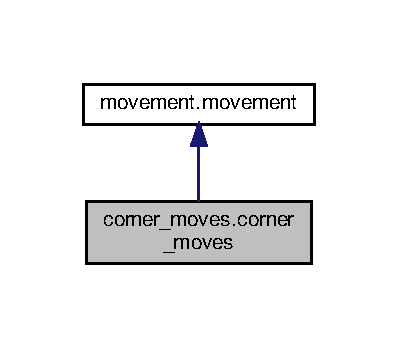
\includegraphics[width=191pt]{classcorner__moves_1_1corner__moves__inherit__graph}
\end{center}
\end{figure}


Collaboration diagram for corner\+\_\+moves.\+corner\+\_\+moves\+:
\nopagebreak
\begin{figure}[H]
\begin{center}
\leavevmode
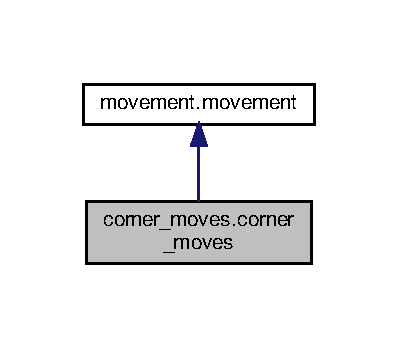
\includegraphics[width=191pt]{classcorner__moves_1_1corner__moves__coll__graph}
\end{center}
\end{figure}
\subsection*{Public Member Functions}
\begin{DoxyCompactItemize}
\item 
def \hyperlink{classcorner__moves_1_1corner__moves_ab52986603fbba7dfcf7d7a824fee483e}{mutation} (self, structure\+\_\+grid)
\item 
def \hyperlink{classcorner__moves_1_1corner__moves_a71da897f349e236a2b89ce47d6f71a75}{\+\_\+\+\_\+init\+\_\+\+\_\+} (self, res, i)
\end{DoxyCompactItemize}
\subsection*{Public Attributes}
\begin{DoxyCompactItemize}
\item 
\mbox{\Hypertarget{classcorner__moves_1_1corner__moves_aff78eb5369bc6db1648731ad805f62ba}\label{classcorner__moves_1_1corner__moves_aff78eb5369bc6db1648731ad805f62ba}} 
{\bfseries residu}
\end{DoxyCompactItemize}


\subsection{Detailed Description}
\begin{DoxyVerb}To be possible, the two connected neighbours of some residue i must
be mutually adjacent to another, unoccupied position on the lattice.
\end{DoxyVerb}
 

\subsection{Constructor \& Destructor Documentation}
\mbox{\Hypertarget{classcorner__moves_1_1corner__moves_a71da897f349e236a2b89ce47d6f71a75}\label{classcorner__moves_1_1corner__moves_a71da897f349e236a2b89ce47d6f71a75}} 
\index{corner\+\_\+moves\+::corner\+\_\+moves@{corner\+\_\+moves\+::corner\+\_\+moves}!\+\_\+\+\_\+init\+\_\+\+\_\+@{\+\_\+\+\_\+init\+\_\+\+\_\+}}
\index{\+\_\+\+\_\+init\+\_\+\+\_\+@{\+\_\+\+\_\+init\+\_\+\+\_\+}!corner\+\_\+moves\+::corner\+\_\+moves@{corner\+\_\+moves\+::corner\+\_\+moves}}
\subsubsection{\texorpdfstring{\+\_\+\+\_\+init\+\_\+\+\_\+()}{\_\_init\_\_()}}
{\footnotesize\ttfamily def corner\+\_\+moves.\+corner\+\_\+moves.\+\_\+\+\_\+init\+\_\+\+\_\+ (\begin{DoxyParamCaption}\item[{}]{self,  }\item[{}]{res,  }\item[{}]{i }\end{DoxyParamCaption})}

\begin{DoxyVerb}Initialize the object corner_moves
    @param res: residu object
    @param   i: index of the residu object
\end{DoxyVerb}
 

\subsection{Member Function Documentation}
\mbox{\Hypertarget{classcorner__moves_1_1corner__moves_ab52986603fbba7dfcf7d7a824fee483e}\label{classcorner__moves_1_1corner__moves_ab52986603fbba7dfcf7d7a824fee483e}} 
\index{corner\+\_\+moves\+::corner\+\_\+moves@{corner\+\_\+moves\+::corner\+\_\+moves}!mutation@{mutation}}
\index{mutation@{mutation}!corner\+\_\+moves\+::corner\+\_\+moves@{corner\+\_\+moves\+::corner\+\_\+moves}}
\subsubsection{\texorpdfstring{mutation()}{mutation()}}
{\footnotesize\ttfamily def corner\+\_\+moves.\+corner\+\_\+moves.\+mutation (\begin{DoxyParamCaption}\item[{}]{self,  }\item[{}]{structure\+\_\+grid }\end{DoxyParamCaption})}

\begin{DoxyVerb}Search the unoccupied position for the movement
    @param structure_grid: A list of lists, which contains the
                    conformation of the sequence
    Return the solution or None if the movement is not possible
\end{DoxyVerb}
 

The documentation for this class was generated from the following file\+:\begin{DoxyCompactItemize}
\item 
/mnt/1373\+B05003\+C22\+A1\+C/\+Scolaire/\+Master/\+M2/projet\+\_\+court/\+R\+E\+M\+C/src/corner\+\_\+moves.\+py\end{DoxyCompactItemize}

\hypertarget{classcrankshaft__moves_1_1crankshaft__moves}{}\section{crankshaft\+\_\+moves.\+crankshaft\+\_\+moves Class Reference}
\label{classcrankshaft__moves_1_1crankshaft__moves}\index{crankshaft\+\_\+moves.\+crankshaft\+\_\+moves@{crankshaft\+\_\+moves.\+crankshaft\+\_\+moves}}


Inheritance diagram for crankshaft\+\_\+moves.\+crankshaft\+\_\+moves\+:
\nopagebreak
\begin{figure}[H]
\begin{center}
\leavevmode
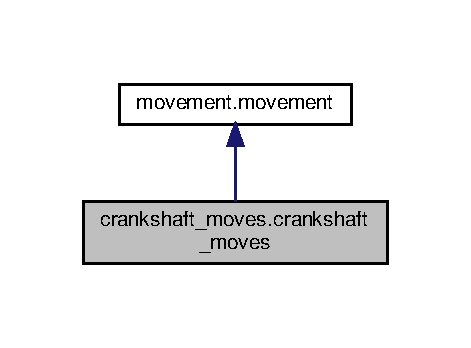
\includegraphics[width=226pt]{classcrankshaft__moves_1_1crankshaft__moves__inherit__graph}
\end{center}
\end{figure}


Collaboration diagram for crankshaft\+\_\+moves.\+crankshaft\+\_\+moves\+:
\nopagebreak
\begin{figure}[H]
\begin{center}
\leavevmode
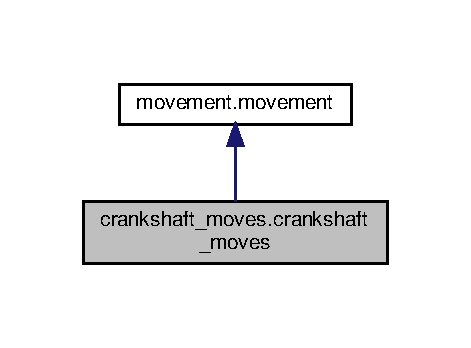
\includegraphics[width=226pt]{classcrankshaft__moves_1_1crankshaft__moves__coll__graph}
\end{center}
\end{figure}
\subsection*{Public Member Functions}
\begin{DoxyCompactItemize}
\item 
def \hyperlink{classcrankshaft__moves_1_1crankshaft__moves_a3f03860d511fcb97e6dd85f851a37c63}{mutation} (self, structure\+\_\+grid)
\item 
def \hyperlink{classcrankshaft__moves_1_1crankshaft__moves_a3d64490ab0dc61e8909c11c65555f512}{\+\_\+\+\_\+init\+\_\+\+\_\+} (self, res, i)
\end{DoxyCompactItemize}
\subsection*{Public Attributes}
\begin{DoxyCompactItemize}
\item 
\mbox{\Hypertarget{classcrankshaft__moves_1_1crankshaft__moves_a379f86aba6d320c666ba363aeb345a1a}\label{classcrankshaft__moves_1_1crankshaft__moves_a379f86aba6d320c666ba363aeb345a1a}} 
{\bfseries residu}
\end{DoxyCompactItemize}


\subsection{Detailed Description}
\begin{DoxyVerb}To be possible, residue i is part of a u-shaped bend in the chain which
involves a 180° rotation of a u-shaped structure consisting
of four connected neighbours.
\end{DoxyVerb}
 

\subsection{Constructor \& Destructor Documentation}
\mbox{\Hypertarget{classcrankshaft__moves_1_1crankshaft__moves_a3d64490ab0dc61e8909c11c65555f512}\label{classcrankshaft__moves_1_1crankshaft__moves_a3d64490ab0dc61e8909c11c65555f512}} 
\index{crankshaft\+\_\+moves\+::crankshaft\+\_\+moves@{crankshaft\+\_\+moves\+::crankshaft\+\_\+moves}!\+\_\+\+\_\+init\+\_\+\+\_\+@{\+\_\+\+\_\+init\+\_\+\+\_\+}}
\index{\+\_\+\+\_\+init\+\_\+\+\_\+@{\+\_\+\+\_\+init\+\_\+\+\_\+}!crankshaft\+\_\+moves\+::crankshaft\+\_\+moves@{crankshaft\+\_\+moves\+::crankshaft\+\_\+moves}}
\subsubsection{\texorpdfstring{\+\_\+\+\_\+init\+\_\+\+\_\+()}{\_\_init\_\_()}}
{\footnotesize\ttfamily def crankshaft\+\_\+moves.\+crankshaft\+\_\+moves.\+\_\+\+\_\+init\+\_\+\+\_\+ (\begin{DoxyParamCaption}\item[{}]{self,  }\item[{}]{res,  }\item[{}]{i }\end{DoxyParamCaption})}

\begin{DoxyVerb}Initialize the object crankshaft_moves
    @param res: residu object
    @param   i: index of the residu object
\end{DoxyVerb}
 

\subsection{Member Function Documentation}
\mbox{\Hypertarget{classcrankshaft__moves_1_1crankshaft__moves_a3f03860d511fcb97e6dd85f851a37c63}\label{classcrankshaft__moves_1_1crankshaft__moves_a3f03860d511fcb97e6dd85f851a37c63}} 
\index{crankshaft\+\_\+moves\+::crankshaft\+\_\+moves@{crankshaft\+\_\+moves\+::crankshaft\+\_\+moves}!mutation@{mutation}}
\index{mutation@{mutation}!crankshaft\+\_\+moves\+::crankshaft\+\_\+moves@{crankshaft\+\_\+moves\+::crankshaft\+\_\+moves}}
\subsubsection{\texorpdfstring{mutation()}{mutation()}}
{\footnotesize\ttfamily def crankshaft\+\_\+moves.\+crankshaft\+\_\+moves.\+mutation (\begin{DoxyParamCaption}\item[{}]{self,  }\item[{}]{structure\+\_\+grid }\end{DoxyParamCaption})}

\begin{DoxyVerb}Search if the residu i is part of a u-shaped then search the
rotation
    @param structure_grid: A list of lists, which contains the
                   conformation of the sequence
    Return the 2 free neighbour in a list
\end{DoxyVerb}
 

The documentation for this class was generated from the following file\+:\begin{DoxyCompactItemize}
\item 
/mnt/1373\+B05003\+C22\+A1\+C/\+Scolaire/\+Master/\+M2/projet\+\_\+court/\+R\+E\+M\+C/src/crankshaft\+\_\+moves.\+py\end{DoxyCompactItemize}

\hypertarget{classend__moves_1_1end__moves}{}\section{end\+\_\+moves.\+end\+\_\+moves Class Reference}
\label{classend__moves_1_1end__moves}\index{end\+\_\+moves.\+end\+\_\+moves@{end\+\_\+moves.\+end\+\_\+moves}}


Inheritance diagram for end\+\_\+moves.\+end\+\_\+moves\+:
\nopagebreak
\begin{figure}[H]
\begin{center}
\leavevmode
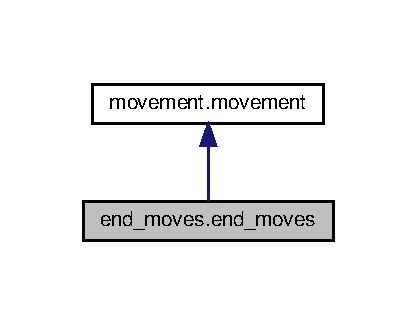
\includegraphics[width=200pt]{classend__moves_1_1end__moves__inherit__graph}
\end{center}
\end{figure}


Collaboration diagram for end\+\_\+moves.\+end\+\_\+moves\+:
\nopagebreak
\begin{figure}[H]
\begin{center}
\leavevmode
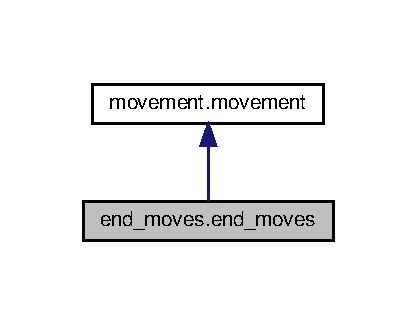
\includegraphics[width=200pt]{classend__moves_1_1end__moves__coll__graph}
\end{center}
\end{figure}
\subsection*{Public Member Functions}
\begin{DoxyCompactItemize}
\item 
def \hyperlink{classend__moves_1_1end__moves_a00ac085203fdadc358c917e4928516c1}{mutation} (self, structure\+\_\+grid)
\item 
def \hyperlink{classend__moves_1_1end__moves_a51b866345b6fb9f3679406b7e26f8d9e}{\+\_\+\+\_\+init\+\_\+\+\_\+} (self, res, i)
\end{DoxyCompactItemize}
\subsection*{Public Attributes}
\begin{DoxyCompactItemize}
\item 
\mbox{\Hypertarget{classend__moves_1_1end__moves_a35b63bb85c918a47bd9ad7247df8b99b}\label{classend__moves_1_1end__moves_a35b63bb85c918a47bd9ad7247df8b99b}} 
{\bfseries index}
\item 
\mbox{\Hypertarget{classend__moves_1_1end__moves_a19dbe2b32973821ca27ecd9a3c4e1caa}\label{classend__moves_1_1end__moves_a19dbe2b32973821ca27ecd9a3c4e1caa}} 
{\bfseries residu}
\end{DoxyCompactItemize}


\subsection{Detailed Description}
\begin{DoxyVerb}The residue is pivoted relative to its connected
neighbour to a free position adjacent to that neighbour.
\end{DoxyVerb}
 

\subsection{Constructor \& Destructor Documentation}
\mbox{\Hypertarget{classend__moves_1_1end__moves_a51b866345b6fb9f3679406b7e26f8d9e}\label{classend__moves_1_1end__moves_a51b866345b6fb9f3679406b7e26f8d9e}} 
\index{end\+\_\+moves\+::end\+\_\+moves@{end\+\_\+moves\+::end\+\_\+moves}!\+\_\+\+\_\+init\+\_\+\+\_\+@{\+\_\+\+\_\+init\+\_\+\+\_\+}}
\index{\+\_\+\+\_\+init\+\_\+\+\_\+@{\+\_\+\+\_\+init\+\_\+\+\_\+}!end\+\_\+moves\+::end\+\_\+moves@{end\+\_\+moves\+::end\+\_\+moves}}
\subsubsection{\texorpdfstring{\+\_\+\+\_\+init\+\_\+\+\_\+()}{\_\_init\_\_()}}
{\footnotesize\ttfamily def end\+\_\+moves.\+end\+\_\+moves.\+\_\+\+\_\+init\+\_\+\+\_\+ (\begin{DoxyParamCaption}\item[{}]{self,  }\item[{}]{res,  }\item[{}]{i }\end{DoxyParamCaption})}

\begin{DoxyVerb}Initialize the object end_moves
    :param res: residu object
    :param   i: index of the residu object
\end{DoxyVerb}
 

\subsection{Member Function Documentation}
\mbox{\Hypertarget{classend__moves_1_1end__moves_a00ac085203fdadc358c917e4928516c1}\label{classend__moves_1_1end__moves_a00ac085203fdadc358c917e4928516c1}} 
\index{end\+\_\+moves\+::end\+\_\+moves@{end\+\_\+moves\+::end\+\_\+moves}!mutation@{mutation}}
\index{mutation@{mutation}!end\+\_\+moves\+::end\+\_\+moves@{end\+\_\+moves\+::end\+\_\+moves}}
\subsubsection{\texorpdfstring{mutation()}{mutation()}}
{\footnotesize\ttfamily def end\+\_\+moves.\+end\+\_\+moves.\+mutation (\begin{DoxyParamCaption}\item[{}]{self,  }\item[{}]{structure\+\_\+grid }\end{DoxyParamCaption})}

\begin{DoxyVerb}Search free neighbour for the residu adjacent.
If several positions are free, one is chosen randomly and the residu
is pivoted to this position.
    @param: structure_grid: A list of lists, which contains the
                   conformation of the sequence
    Return None if the movement is not possible or the free position
\end{DoxyVerb}
 

The documentation for this class was generated from the following file\+:\begin{DoxyCompactItemize}
\item 
/mnt/1373\+B05003\+C22\+A1\+C/\+Scolaire/\+Master/\+M2/projet\+\_\+court/\+R\+E\+M\+C/src/end\+\_\+moves.\+py\end{DoxyCompactItemize}

\hypertarget{classmovement_1_1movement}{}\section{movement.\+movement Class Reference}
\label{classmovement_1_1movement}\index{movement.\+movement@{movement.\+movement}}


Inheritance diagram for movement.\+movement\+:
\nopagebreak
\begin{figure}[H]
\begin{center}
\leavevmode
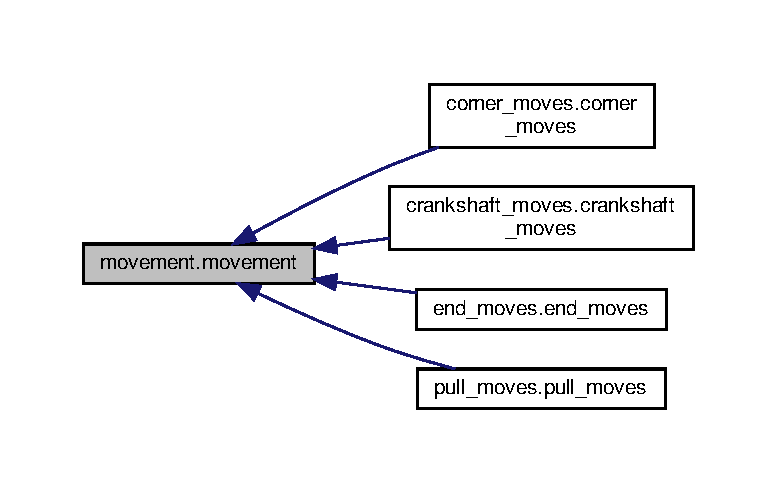
\includegraphics[width=350pt]{classmovement_1_1movement__inherit__graph}
\end{center}
\end{figure}
\subsection*{Public Member Functions}
\begin{DoxyCompactItemize}
\item 
def \hyperlink{classmovement_1_1movement_aeaf128c02480726c4018c5df71d96813}{count\+Bonds} (self, structure\+\_\+grid, residues)
\item 
def \hyperlink{classmovement_1_1movement_a6d04cb00a64e07aa940a60b726c4f435}{change\+Oneresidu} (self, structure\+\_\+grid, residues, random\+\_\+neighbour)
\item 
def \hyperlink{classmovement_1_1movement_aa403a41df1f55760dd5581c167f03a0c}{change\+Tworesidues} (self, structure\+\_\+grid, residues, random\+\_\+neighbour)
\item 
def \hyperlink{classmovement_1_1movement_acf4e8b0e3c24c68bde44e1d66820dc41}{\+\_\+\+\_\+init\+\_\+\+\_\+} (self, i)
\end{DoxyCompactItemize}
\subsection*{Public Attributes}
\begin{DoxyCompactItemize}
\item 
\mbox{\Hypertarget{classmovement_1_1movement_a4923d729a062d560c3f549a20569d7e4}\label{classmovement_1_1movement_a4923d729a062d560c3f549a20569d7e4}} 
{\bfseries index}
\end{DoxyCompactItemize}


\subsection{Detailed Description}
\begin{DoxyVerb}Mother class of all movements.
\end{DoxyVerb}
 

\subsection{Constructor \& Destructor Documentation}
\mbox{\Hypertarget{classmovement_1_1movement_acf4e8b0e3c24c68bde44e1d66820dc41}\label{classmovement_1_1movement_acf4e8b0e3c24c68bde44e1d66820dc41}} 
\index{movement\+::movement@{movement\+::movement}!\+\_\+\+\_\+init\+\_\+\+\_\+@{\+\_\+\+\_\+init\+\_\+\+\_\+}}
\index{\+\_\+\+\_\+init\+\_\+\+\_\+@{\+\_\+\+\_\+init\+\_\+\+\_\+}!movement\+::movement@{movement\+::movement}}
\subsubsection{\texorpdfstring{\+\_\+\+\_\+init\+\_\+\+\_\+()}{\_\_init\_\_()}}
{\footnotesize\ttfamily def movement.\+movement.\+\_\+\+\_\+init\+\_\+\+\_\+ (\begin{DoxyParamCaption}\item[{}]{self,  }\item[{}]{i }\end{DoxyParamCaption})}

\begin{DoxyVerb}Initialize the object movement
    @param   i: index of the residu object
\end{DoxyVerb}
 

\subsection{Member Function Documentation}
\mbox{\Hypertarget{classmovement_1_1movement_a6d04cb00a64e07aa940a60b726c4f435}\label{classmovement_1_1movement_a6d04cb00a64e07aa940a60b726c4f435}} 
\index{movement\+::movement@{movement\+::movement}!change\+Oneresidu@{change\+Oneresidu}}
\index{change\+Oneresidu@{change\+Oneresidu}!movement\+::movement@{movement\+::movement}}
\subsubsection{\texorpdfstring{change\+Oneresidu()}{changeOneresidu()}}
{\footnotesize\ttfamily def movement.\+movement.\+change\+Oneresidu (\begin{DoxyParamCaption}\item[{}]{self,  }\item[{}]{structure\+\_\+grid,  }\item[{}]{residues,  }\item[{}]{random\+\_\+neighbour }\end{DoxyParamCaption})}

\begin{DoxyVerb}Change the conformation of one residu.
    @param: structure_grid: A list of lists, which contains the
                   conformation of the sequence
    @param residues: A list of residu object
    @param random_neighbour: A dictionnary with coordinates of
                     the free position
    Return the new conformation and residues obejct modified.
\end{DoxyVerb}
 \mbox{\Hypertarget{classmovement_1_1movement_aa403a41df1f55760dd5581c167f03a0c}\label{classmovement_1_1movement_aa403a41df1f55760dd5581c167f03a0c}} 
\index{movement\+::movement@{movement\+::movement}!change\+Tworesidues@{change\+Tworesidues}}
\index{change\+Tworesidues@{change\+Tworesidues}!movement\+::movement@{movement\+::movement}}
\subsubsection{\texorpdfstring{change\+Tworesidues()}{changeTworesidues()}}
{\footnotesize\ttfamily def movement.\+movement.\+change\+Tworesidues (\begin{DoxyParamCaption}\item[{}]{self,  }\item[{}]{structure\+\_\+grid,  }\item[{}]{residues,  }\item[{}]{random\+\_\+neighbour }\end{DoxyParamCaption})}

\begin{DoxyVerb}Change the conformation of two residues.
    @param: structure_grid: A list of lists, which contains the
                   conformation of the sequence
    @param residues: A list of residu object
    @param random_neighbour: A list with 2 dictionnaries containing
                     coordinates of the 2 free positions and
                     the difference between the 2 residues
                     to move
    Return the new conformation and reidues objet modified.
\end{DoxyVerb}
 \mbox{\Hypertarget{classmovement_1_1movement_aeaf128c02480726c4018c5df71d96813}\label{classmovement_1_1movement_aeaf128c02480726c4018c5df71d96813}} 
\index{movement\+::movement@{movement\+::movement}!count\+Bonds@{count\+Bonds}}
\index{count\+Bonds@{count\+Bonds}!movement\+::movement@{movement\+::movement}}
\subsubsection{\texorpdfstring{count\+Bonds()}{countBonds()}}
{\footnotesize\ttfamily def movement.\+movement.\+count\+Bonds (\begin{DoxyParamCaption}\item[{}]{self,  }\item[{}]{structure\+\_\+grid,  }\item[{}]{residues }\end{DoxyParamCaption})}

\begin{DoxyVerb}Counts the number of bonds. For each bond, an energy of -1 is
summed.
    @param: structure_grid: A list of lists, which contains the
                   conformation of the sequence
    @param residues: A list of residu object
    Return the total energy.
\end{DoxyVerb}
 

The documentation for this class was generated from the following file\+:\begin{DoxyCompactItemize}
\item 
/mnt/1373\+B05003\+C22\+A1\+C/\+Scolaire/\+Master/\+M2/projet\+\_\+court/\+R\+E\+M\+C/src/movement.\+py\end{DoxyCompactItemize}

\hypertarget{classpull__moves_1_1pull__moves}{}\section{pull\+\_\+moves.\+pull\+\_\+moves Class Reference}
\label{classpull__moves_1_1pull__moves}\index{pull\+\_\+moves.\+pull\+\_\+moves@{pull\+\_\+moves.\+pull\+\_\+moves}}


Inheritance diagram for pull\+\_\+moves.\+pull\+\_\+moves\+:
\nopagebreak
\begin{figure}[H]
\begin{center}
\leavevmode
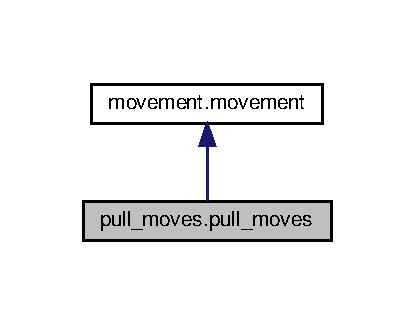
\includegraphics[width=199pt]{classpull__moves_1_1pull__moves__inherit__graph}
\end{center}
\end{figure}


Collaboration diagram for pull\+\_\+moves.\+pull\+\_\+moves\+:
\nopagebreak
\begin{figure}[H]
\begin{center}
\leavevmode
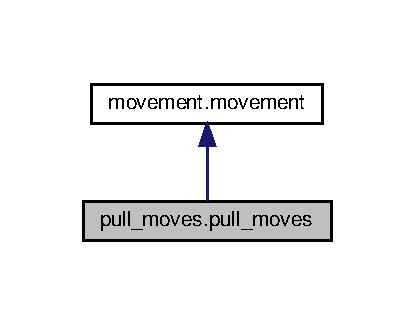
\includegraphics[width=199pt]{classpull__moves_1_1pull__moves__coll__graph}
\end{center}
\end{figure}
\subsection*{Public Member Functions}
\begin{DoxyCompactItemize}
\item 
def \hyperlink{classpull__moves_1_1pull__moves_a2322051e5c24802bdcda8604e7a00b20}{mutation} (self, structure\+\_\+grid, residues)
\item 
def \hyperlink{classpull__moves_1_1pull__moves_a0877c3a2c3818eecdf3622ea01acf714}{\+\_\+\+\_\+init\+\_\+\+\_\+} (self, res, i)
\end{DoxyCompactItemize}
\subsection*{Public Attributes}
\begin{DoxyCompactItemize}
\item 
\mbox{\Hypertarget{classpull__moves_1_1pull__moves_a09866746bd2414da818ba8eedb1963ac}\label{classpull__moves_1_1pull__moves_a09866746bd2414da818ba8eedb1963ac}} 
{\bfseries residu}
\end{DoxyCompactItemize}


\subsection{Detailed Description}
\begin{DoxyVerb}A square is formed by residues i, i + 1, L and C.
A pull move can only proceed if C is either empty or occupied by
residue i - 1.
\end{DoxyVerb}
 

\subsection{Constructor \& Destructor Documentation}
\mbox{\Hypertarget{classpull__moves_1_1pull__moves_a0877c3a2c3818eecdf3622ea01acf714}\label{classpull__moves_1_1pull__moves_a0877c3a2c3818eecdf3622ea01acf714}} 
\index{pull\+\_\+moves\+::pull\+\_\+moves@{pull\+\_\+moves\+::pull\+\_\+moves}!\+\_\+\+\_\+init\+\_\+\+\_\+@{\+\_\+\+\_\+init\+\_\+\+\_\+}}
\index{\+\_\+\+\_\+init\+\_\+\+\_\+@{\+\_\+\+\_\+init\+\_\+\+\_\+}!pull\+\_\+moves\+::pull\+\_\+moves@{pull\+\_\+moves\+::pull\+\_\+moves}}
\subsubsection{\texorpdfstring{\+\_\+\+\_\+init\+\_\+\+\_\+()}{\_\_init\_\_()}}
{\footnotesize\ttfamily def pull\+\_\+moves.\+pull\+\_\+moves.\+\_\+\+\_\+init\+\_\+\+\_\+ (\begin{DoxyParamCaption}\item[{}]{self,  }\item[{}]{res,  }\item[{}]{i }\end{DoxyParamCaption})}

\begin{DoxyVerb}Initialize the object end_moves
    @param res: residu object
    @param   i: index of the residu object
\end{DoxyVerb}
 

\subsection{Member Function Documentation}
\mbox{\Hypertarget{classpull__moves_1_1pull__moves_a2322051e5c24802bdcda8604e7a00b20}\label{classpull__moves_1_1pull__moves_a2322051e5c24802bdcda8604e7a00b20}} 
\index{pull\+\_\+moves\+::pull\+\_\+moves@{pull\+\_\+moves\+::pull\+\_\+moves}!mutation@{mutation}}
\index{mutation@{mutation}!pull\+\_\+moves\+::pull\+\_\+moves@{pull\+\_\+moves\+::pull\+\_\+moves}}
\subsubsection{\texorpdfstring{mutation()}{mutation()}}
{\footnotesize\ttfamily def pull\+\_\+moves.\+pull\+\_\+moves.\+mutation (\begin{DoxyParamCaption}\item[{}]{self,  }\item[{}]{structure\+\_\+grid,  }\item[{}]{residues }\end{DoxyParamCaption})}

\begin{DoxyVerb}Check if the conformation is correct to do the pull move.
If so, return the 2 new positions in a list.
    @param structure_grid: A list of lists, which contains the
                   conformation of the sequence
    @param residues: A list of residu object
    Return None if the movement is not possible or return the 2
positions and the second residu to move
\end{DoxyVerb}
 

The documentation for this class was generated from the following file\+:\begin{DoxyCompactItemize}
\item 
/mnt/1373\+B05003\+C22\+A1\+C/\+Scolaire/\+Master/\+M2/projet\+\_\+court/\+R\+E\+M\+C/src/pull\+\_\+moves.\+py\end{DoxyCompactItemize}

\hypertarget{classresidu_1_1residu}{}\section{residu.\+residu Class Reference}
\label{classresidu_1_1residu}\index{residu.\+residu@{residu.\+residu}}
\subsection*{Public Member Functions}
\begin{DoxyCompactItemize}
\item 
def \hyperlink{classresidu_1_1residu_a63505767ea98b9e6e17196019c07ce1b}{search\+\_\+free\+\_\+neighbour} (self, structure\+\_\+grid)
\item 
def \hyperlink{classresidu_1_1residu_a30216b9f76412426033dcd14fadad9e4}{\+\_\+\+\_\+init\+\_\+\+\_\+} (self, hydrophobicity, x, y)
\end{DoxyCompactItemize}
\subsection*{Public Attributes}
\begin{DoxyCompactItemize}
\item 
\mbox{\Hypertarget{classresidu_1_1residu_afc7d129ad064dfec120862d4426f8e24}\label{classresidu_1_1residu_afc7d129ad064dfec120862d4426f8e24}} 
{\bfseries hp}
\item 
\mbox{\Hypertarget{classresidu_1_1residu_afa338fe84f0d017a0d23d018835897ee}\label{classresidu_1_1residu_afa338fe84f0d017a0d23d018835897ee}} 
{\bfseries line}
\item 
\mbox{\Hypertarget{classresidu_1_1residu_aef02a7e46e5cdbbf4190ebfc45b09206}\label{classresidu_1_1residu_aef02a7e46e5cdbbf4190ebfc45b09206}} 
{\bfseries column}
\end{DoxyCompactItemize}


\subsection{Detailed Description}
\begin{DoxyVerb}A class containing the coordinates of one amino acid and its
hydrophobicty. It contains its previous and next residu in the sequence.
\end{DoxyVerb}
 

\subsection{Constructor \& Destructor Documentation}
\mbox{\Hypertarget{classresidu_1_1residu_a30216b9f76412426033dcd14fadad9e4}\label{classresidu_1_1residu_a30216b9f76412426033dcd14fadad9e4}} 
\index{residu\+::residu@{residu\+::residu}!\+\_\+\+\_\+init\+\_\+\+\_\+@{\+\_\+\+\_\+init\+\_\+\+\_\+}}
\index{\+\_\+\+\_\+init\+\_\+\+\_\+@{\+\_\+\+\_\+init\+\_\+\+\_\+}!residu\+::residu@{residu\+::residu}}
\subsubsection{\texorpdfstring{\+\_\+\+\_\+init\+\_\+\+\_\+()}{\_\_init\_\_()}}
{\footnotesize\ttfamily def residu.\+residu.\+\_\+\+\_\+init\+\_\+\+\_\+ (\begin{DoxyParamCaption}\item[{}]{self,  }\item[{}]{hydrophobicity,  }\item[{}]{x,  }\item[{}]{y }\end{DoxyParamCaption})}

\begin{DoxyVerb}Initialize the object residu
    @param hydrophobicty: h or p
    @param   x: the line of the residu
    @param   y: the column of the residu
\end{DoxyVerb}
 

\subsection{Member Function Documentation}
\mbox{\Hypertarget{classresidu_1_1residu_a63505767ea98b9e6e17196019c07ce1b}\label{classresidu_1_1residu_a63505767ea98b9e6e17196019c07ce1b}} 
\index{residu\+::residu@{residu\+::residu}!search\+\_\+free\+\_\+neighbour@{search\+\_\+free\+\_\+neighbour}}
\index{search\+\_\+free\+\_\+neighbour@{search\+\_\+free\+\_\+neighbour}!residu\+::residu@{residu\+::residu}}
\subsubsection{\texorpdfstring{search\+\_\+free\+\_\+neighbour()}{search\_free\_neighbour()}}
{\footnotesize\ttfamily def residu.\+residu.\+search\+\_\+free\+\_\+neighbour (\begin{DoxyParamCaption}\item[{}]{self,  }\item[{}]{structure\+\_\+grid }\end{DoxyParamCaption})}

\begin{DoxyVerb}Search for freedom neighbour and return a dictionnaire
of their coordinates
\end{DoxyVerb}
 

The documentation for this class was generated from the following file\+:\begin{DoxyCompactItemize}
\item 
/mnt/1373\+B05003\+C22\+A1\+C/\+Scolaire/\+Master/\+M2/projet\+\_\+court/\+R\+E\+M\+C/src/residu.\+py\end{DoxyCompactItemize}

%--- End generated contents ---

% Index
\backmatter
\newpage
\phantomsection
\clearemptydoublepage
\addcontentsline{toc}{chapter}{Index}
\printindex

\end{document}
